\documentclass[a4paper,12pt]{article}
\usepackage{graphicx}
\graphicspath{ {images/} }

% Language and font encodings
\usepackage[utf8]{inputenc}
\usepackage[american]{babel}

% Specify bibliography package
\usepackage{csquotes}% Recommended
\usepackage[style=apa]{biblatex}
\DeclareLanguageMapping{american}{american-apa}
\addbibresource{references.bib}

% Sets page size and margins
\usepackage[top=2cm,bottom=2cm,left=2cm,right=2cm,marginparwidth=1.75cm]{geometry}
\setlength{\parskip}{1em}

% package for formatting and highlighting source code
\usepackage{listings}
\usepackage{color}

% Useful packages
\usepackage{amsmath}
\usepackage{graphicx}
\usepackage{float}
\usepackage[colorlinks=true, allcolors=black]{hyperref}
\usepackage{graphicx}
\usepackage{setspace}

% packages for tikz diagrams
\usepackage{tikz}
\usetikzlibrary{shapes.geometric, arrows}

% styling for tikz diagrams
\tikzstyle{startstop} = [rectangle, rounded corners, minimum width=10cm, minimum height=1cm,text centered, text width=10cm, draw=black, fill=gray!10]
\tikzstyle{process} = [rectangle, minimum width=10cm, minimum height=1cm, text centered, text width=10cm, draw=black, fill=orange!30]
\tikzstyle{arrow} = [thick,->,>=stealth]

% List of abbreviations
\usepackage {acronym}

% Section Title Margins
\usepackage{titlesec}
\titlespacing*{\section}
{0pt}{3.0ex plus 1ex minus .2ex}{0.7ex}
\titlespacing*{\subsection}
{0pt}{1.4ex}{0pt}
\definecolor{dkgreen}{rgb}{0,0.6,0}
\definecolor{gray}{rgb}{0.5,0.5,0.5}
\definecolor{mauve}{rgb}{0.58,0,0.82}

\lstset{frame=tb,
  language=Python,
  aboveskip=3mm,
  belowskip=3mm,
  showstringspaces=false,
  columns=flexible,
  basicstyle={\small\ttfamily},
  numbers=none,
  numberstyle=\tiny\color{gray},
  keywordstyle=\color{blue},
  commentstyle=\color{dkgreen},
  stringstyle=\color{mauve},
  breaklines=true,
  breakatwhitespace=true,
  tabsize=3}

\title{Your Title Goes Here}
\author{Your Name Goes Here}

%************************** DOCUMENT_STARTS_HERE **************************
\begin{document}

\begin{titlepage}
	\begin{figure}
	\centering
	
\includegraphics[scale=0.32]{logohsg}
	\end{figure}
\centering
\centering
{\scshape\large School of Management, Economics, Law, Social Sciences and International Affairs \par}
\vspace{1.7cm}
{\huge\bfseries The effect of Twitter activity on \\ Bitcoin price\par}
\vspace{1.0cm}
{\Huge\itshape Documentation\par}
\vspace{1.0cm}     
{\Large Software Engineering for Economists \\ (7,610,1.00) \par}
\vspace{1.2cm}
{Alen Stepic - 11-475-258 \\ Dimitrios Koumnakes - 10-613-370 \\ Severin Kranz - 13-606-355 \\ Joël Sonderegger - 11-495-488 \\ Chi Xu - 16-300-915 \par}
\vspace{1.2cm}
Fall Term 2017 \\
\vspace{1.2cm}
{Supervisor:\\ Prof. Dr. Philipp Zahn\\ FGN HSG\\ Varnbüelstrasse 19\\ 9000 St. Gallen\\ Department of Economics\par}
\vspace{0.8cm}
{\centering\today\par}
\end{titlepage}

\clearpage

\tableofcontents

\clearpage
    
\listoffigures\bigskip 
\section*{List of Abbreviations} 
\begin{acronym}[ASECRETTT]
\acro{API}{Application Programming Interface}
\acro{ATOKEN}{Access Token}
\acro{ASECRET}{Access Token Secret}
\acro{BPI}{Bitcoin Price Index}
\acro{BTC}{Bitcoin}
\acro{CKEY}{Consumer Key}
\acro{CSECRET}{Consumer Secret}
\acro{JSON}{Java Script Object Notation}
\acro{RPI}{Raspberry Pi}
\acro{SSH}{Secure Shell}
\acro{USD}{US Dollar}
\end{acronym}

\clearpage

\begin{spacing}{1.2}
\cleardoublepage\pagenumbering{arabic}

\section{Introduction}
In the academic environment both accountability and reproducibility are important to ensure a high quality of research. However, the publishing process of scientific papers and journals seems to be outdated, as reproducibility is not evaluated by leading journals. \parencite[p.~888]{mccullough2003} Driven by digitalization, new ways of data collection and processing arise by using high computational capacity and advanced econometric methods. On the one hand, the usage of scripts, automation or machine learning can increase effectiveness and efficiency. Hence, much larger data sets can be proceeded. On the other hand, this creates also new challenges to trace and reproduce data sets, procedures or analysis. There are often cited academic papers, where the initial computation is neither clearly documented nor reproducible \parencite[pp.~874--887]{mccullough2003}. Replicating data or existing results does not provide any new knowledge at all. Nevertheless, the ability to understand what researchers have done is key. Non-reproducible work cannot be characterised as science or used as a basis for policy-making \parencite[p.~888]{mccullough2003}. Therefore, clear documentation of processes, used scripts and tools should be the basis of every scientific publication.

\subsection{Goal}
The objective of this documentation is to provide a detailed description of the research process, used hardware, software, procedures and tools of the accompanying paper. This description enables the reader to reproduce the results discussed in our work. Thus, it contains an explanation of how  input data have been gathered, stored, aggregated and analyzed. 

\subsection{Methodology}
After pointing out the relevance of this documentation, the second chapter is an explanation of the required set-up in order to reproduce our results by running our Python scripts available from Github. The programming language Python has been chosen, as it comes with a high variety of modules and is especially suitable for data science. The third chapter discusses the input data of our project. This includes the process of gathering and storing tweets from Twitter, as well as the collecting Bitcoin price data for the same time frame. Both Twitter and Bitcoin data have been gathered by using an Application Programming Interface (API), which allow to access real-life data by a set of explicitly defined and documented methods. Further on, the fourth chapter explains, how the data has been aggregated and wrangled to enable the subsequent analysis. Finally, the statistical analysis has been conducted with STATA and is discussed in the last chapter of this documentation.

\subsection{Scope}
The scope of the documentation is to provide an overview of the different steps that have been conducted to obtain the results of the paper. Therefore, this documentation includes all information necessary to understand and reproduce our findings from the accompanying paper. However, it does not contain any further information about the content and results of our research and is only meant as supportive material. Furthermore, it does not provide a detailed description of the code itself, in order to avoid redundancy of information with the existing code documentation within the scripts. 
\clearpage

\section{Set-up}
This section goes through the set-up that is necessary in order to execute the code discussed in this documentation.

\subsection{Github repository}
All code is available on the following Github repository:
\newline
\verb|https://github.com/joelsonderegger/twitterbitcoin/|
\subsection{Requirements to run Python scripts}
Before you go any further, make sure that at least Python version 3.0.0 is available from your command line. You can check this by running in your command line:
\begin{lstlisting}[language=bash]
    python --version
\end{lstlisting}

You should get some output like Python 3.7.13. If you do not have at least Python version 3.0.0, please install the latest 3.x version from \verb|python.org|.
\newline \newline
On top, you need various Python packages. We created a requirements file \verb|requirements.txt|, which contains all required packages to run the Python scripts of this project. You can find the \verb|requirements.txt| in the root directory of our Github repository. The list of packages can be installed using pip install like so:

\begin{lstlisting}[language=bash]
    pip install -r requirements.txt
\end{lstlisting}
Now you should be ready to run the Python scripts.

\subsection{STATA}
For the statistical analysis of our data, we used the statistical software STATA (version 14.2). When seeking for statistical analysis, regression analysis or data management, STATA is a capable tool. To reproduce our results, you need to have the STATA software installed on your local computer. After starting the program, you can follow the guidelines in chapter 5 (Data Analysis). 

\clearpage

\section{Data Collection}
The following section contains a detailed description of how the data for the sequential analysis is gathered and stored. Two separate data sets will be collected: (1) Tweets data and (2) Bitcoin price index data.
\subsection{Tweets Data}
With the Python script \verb|collectTwitterData.py| real-time Twitter data are streamed and stored using the Python library Tweepy. A Raspberry Pi can be used to gather Twitter data over a longer period.
\subsubsection{Python Script}
Twitter offers different APIs for the collection of Twitter data. However, the time frame to gather data from the past with full access is limited to seven days \parencite{twitterinc2017a}. To gather a data set over a longer period, without using payed services Twitter, data have to be streamed and saved in real-time. Python offers different Twitter libraries such as the package Tweepy.

\paragraph{Tweepy}\mbox{}\\{}
Tweepy is a open-source libary. It provides a simple way to gather real time tweets, by managing authentication, connection and tweet information of Twitters streaming API. The Tweepy instance tweepy.streaming is used for the streaming session and forwards the data to the StreamListener instance. The \verb|class listener(StreamListener)| calls the method \verb|def on_data(self, data)|. With this method all data of filtered tweets are gathered in real-time. \parencite{tweepy} The main function \verb|def main()| manages the required authentication as follows:
\begin{lstlisting}[language=bash]
auth = OAuthHandler (ckey, csecret)
auth.set_access_token(atoken, asecret)
\end{lstlisting}
Those authentications are demanded by Twitter and explained in more details in the next paragraph. Furthermore, the main function starts to run the stream, while filtering for the buzzword "Bitcoin" by processing \verb|twitterStream.filter(track=["bitcoin"]|. Tweepy has been applied for this project because it simplifies the script and enables its users to gather a huge number of tweets without any costs. 


\paragraph{Installing Tweepy}\mbox{}\\{}
Tweepy is installed easily by running following commands in the command prompt. However, this step should not be necessary if you have previously completed the above described setup using the requirements file \verb|requirements.txt|.
\begin{lstlisting}[language=bash]
pip install tweepy
\end{lstlisting}

If the previously downloaded Python installation package does not contain the tweepy library, the tweepy package has to be downloaded manually. The package can be downloaded for free from the following link:
\begin{lstlisting}[language=bash]
https://pypi.python.org/pypi/tweepy
\end{lstlisting}

\paragraph{Twitter Authentication}\mbox{}\\{}
To access the Twitter data, Twitter requests an identification of the user. The identification is assured by different keys and access tokens. Those are the (1) consumer key (CKEY), (2) consumer secret (CSECRET), (3) access token (ATOKEN) and (4) access token secret (ASECRET). \parencite{twitterinc2017b}

To obtain the mentioned keys and tokens a Twitter account is needed. Once, a Twitter account exists, an application has to be created by logging in the developer area with the credentials under the following link: 
\begin{lstlisting}[language=bash]
https://apps.twitter.com/
\end{lstlisting}

After the creation of an application, the keys and tokens can be extracted. Figure \ref{figkeysandtokens} illustrates how to retrieve the keys and tokens.\\
\begin{figure}[H]
\centering
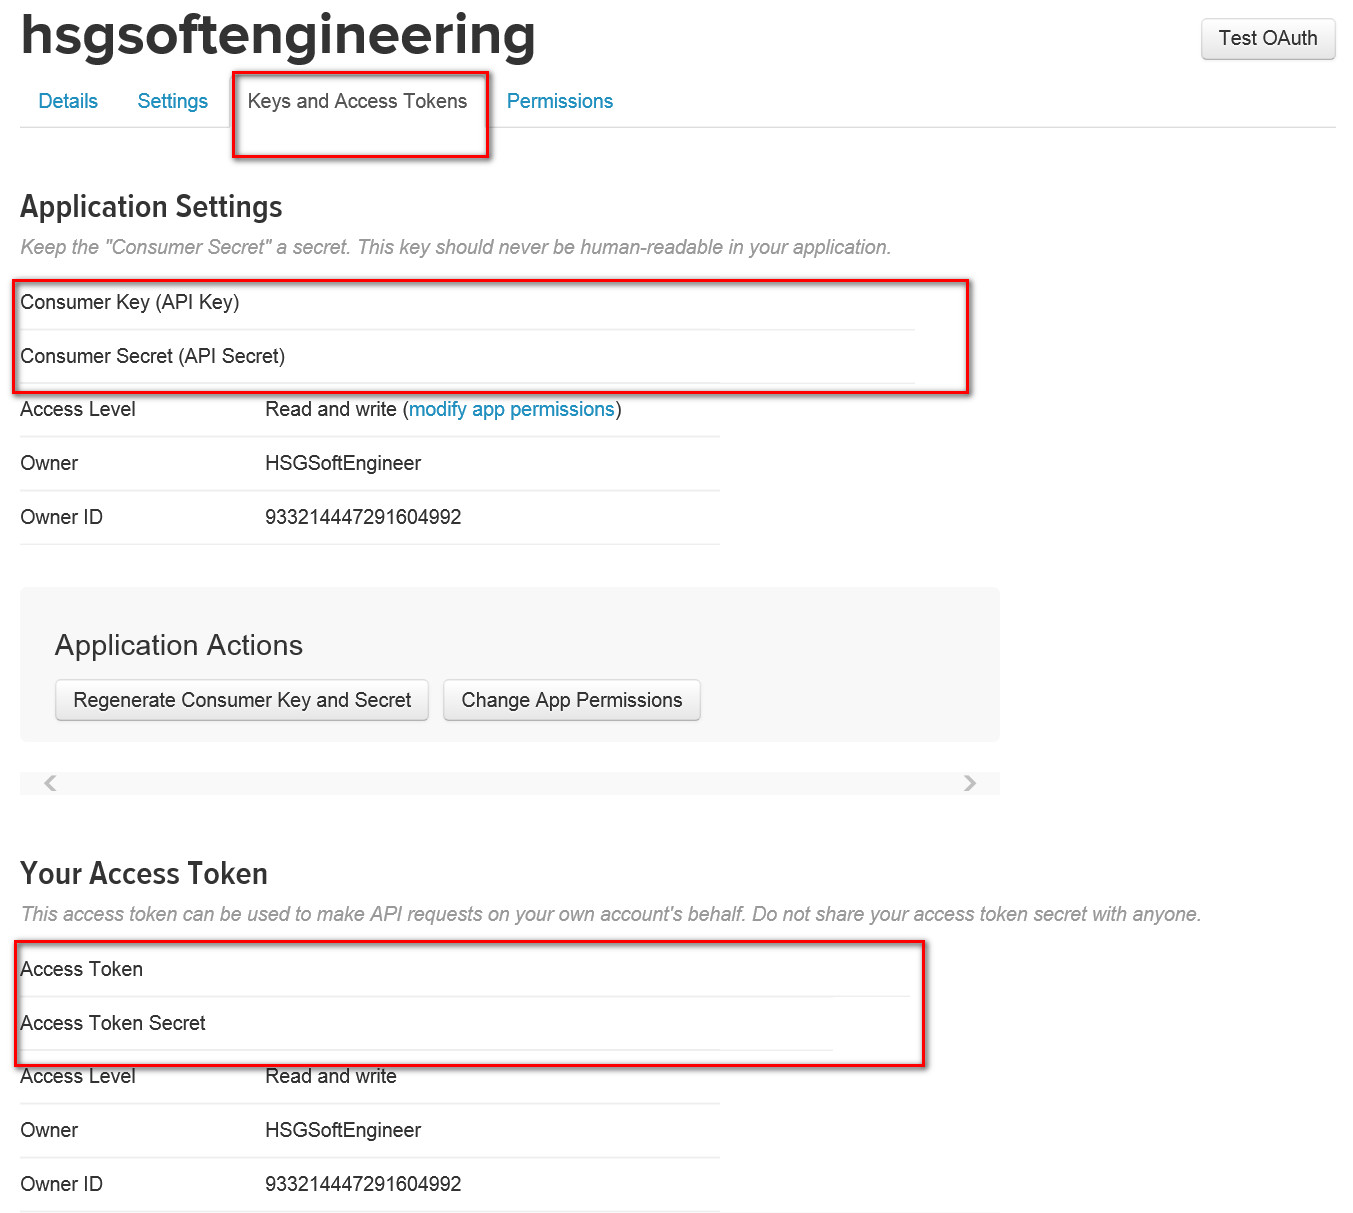
\includegraphics[scale=0.6]{twitteraccess}
\caption{Twitter Keys and Access Tokens, based on \textcite{twitterinc2017c}.}
\label{figkeysandtokens}
\end{figure}

\paragraph{Running the Python Script}\mbox{}\\{}
By running the Python script \verb|collectTwitterData.py| real-time Twitter data is gathered on an ongoing basis until you stop the script forcefully.
\begin{lstlisting}[language=bash]
    $ python collectTwitterData.py
    \end{lstlisting}

The Twitter API provides the tweets data in a Java Script Object Notation (JSON) format. Tweets are only received in case a tweet contains the predefined key word \verb|bitcoin|. While a single tweet consists of many attributes we are only interested in two attributes:
\begin{itemize}
    \item created\_at: Timestamp of the created tweet (in UTC time)
    \item text: Text of the tweet
\end{itemize}

An example for a response from the Tweepy API looks like this (of course this shows only the two attributes we are interested in):
\begin{lstlisting}
    {
        ...
        "created_at": Tue Dec 19 20:40:49 +0000 2017, 
        "text": "Singapore issues bitcoin warning after price rise - #BTC #Bitcoin #Crypto"
        ...
    }
\end{lstlisting}

The \verb|text| attribute needs to be encoded from the raw JSON format into the UTF-8 format for further analysis. After successfully encoding the \verb|text| attribute a tweet is appended to the \verb|twitterData.csv| file as a new row and saved in the /data folder.

To ensure a high quality data set, without missing any data points for the observed period, we have built in an exception handler into the \verb|collectTwitterData.py| script. If an error occurs an email will be sent with the error message. Additionally, any exception that occurs during the execution of the script will be added to the log file \verb|/data/tweet_collection_error_log.csv|.

\subsubsection{Hardware set-up}
As explained in the previous section the Twitter API was used to gather tweets in real-time based on the buzzword "bitcoin" by using Tweepy. The Python script was running for seven days without interruption on a Raspberry Pi 2 (RPI) which was accessed with a Secure Shell (SSH) connection. This approach allowed us to ensure a continuous data stream while being able to access the program output regardless of time and location. Furthermore, due to a low energy consumption of the RPI, the method is also the most cost efficient option compared to a personal computer or NAS Server. The following section describes the different steps that have been taken in order to set up the RPI 2, SSH, Git and Python3.\\

\begin{enumerate}

\item Setup of the Raspberry Pi
\begin{enumerate}
\item Burn image 2017-11-29-raspbian-stretch.zip to micro SD card available from
\begin{lstlisting}[language=bash]
https://www.raspberrypi.org/downloads/raspbian/
\end{lstlisting}
\item Boot image from micro SD card 
\item Open SSH session using PuTTY SSH client for Windows available from
\begin{lstlisting}[language=bash] 
https://www.chiark.greenend.org.uk/~sgtatham/putty/latest.html
\end{lstlisting}
\item Login to server with credentials 
\end{enumerate}

\item Update system to the newest software
\begin{enumerate}
\item Update list of applications with the command
\begin{lstlisting}[language=bash]
sudo apt-get update
\end{lstlisting}
\item Update applications with the command
\begin{lstlisting}[language=bash]
sudo apt-get upgrade
\end{lstlisting}
\end{enumerate}

\item Setup Git
\begin{enumerate}
\item Install Git using the command
\begin{lstlisting}[language=bash]
 sudo apt-get install git
\end{lstlisting}
\item Clone Git repository from
\begin{lstlisting}[language=bash] 
https://github.com/joelsonderegger/twitterbitcoin.git
\end{lstlisting}
\end{enumerate}

\item Setup Python3
\begin{enumerate}
\item Install Python3 using the command: \begin{lstlisting}[language=bash]
sudo apt-get install Python3
\end{lstlisting}
\item Install the tweepy module for Python using the command
\begin{lstlisting}[language=bash]
pip install tweepy
\end{lstlisting}
\end{enumerate}

\item Collect Twitter Data
\begin{enumerate}
\item Open a new screen using the command
\begin{lstlisting}[language=bash] 
screen -S 'name' 
\end{lstlisting}
\item Start Python program using the command
\begin{lstlisting}[language=bash]
python3 collectTwitterData.py
\end{lstlisting}
\item Detach the screen to keep the program running after secure shell connection has been terminated using the commands
\begin{lstlisting}[language=bash]
Ctrl+A
Ctrl+D
\end{lstlisting}
\item Re-attach the screen to check whether the script is still running using the command
\begin{lstlisting}[language=bash]
screen -r 'name'
\end{lstlisting}
\end{enumerate}

\item Download the collected data
\begin{enumerate}
\item Install FileZilla on your local machine available from
\begin{lstlisting}[language=bash] 
https://filezilla-project.org/
\end{lstlisting}
\item Connect to RPI and navigate to data location \newline
\item Download data manually \newline \newline \end{enumerate}
\end{enumerate}

In summary, this approach worked well and ran smoothly. A clean set-up is recommended to ensure a continuous data stream over a longer period.


\subsection{Bitcoin Price Data}
We wrote a Python script which collects Bitcoin price data as there was no pre-existing data set that satisfied our needs. The Bitcoin price is best expressed by the Bitcoin Price Index (\cite{kristoufek2015main}). The Bitcoin price index (BPI) is an index of the exchange rate between the Bitcoin (BTC) and the US dollar (USD). The objective of the script was to gather hourly Bitcoin Price Index data for at least the time period in which we gather the tweets data. We found an API by bitcoinaverage.com which was sufficed our needs. A detailed description of the API follows in section 3.2.3.

\subsubsection{Execution}
By executing the Python script \verb|collectCryptocurrencyData.py| hourly data for the Bitcoin Price Index is retrieved.
\begin{lstlisting}[language=bash]
    $ python collectCryptocurrencyData.py
\end{lstlisting}

\subsubsection{Output}
After successfully running the Python script \verb|CollectCryptocurrencyData.py| the file \verb|bpi.csv| is generated in the folder \verb|/data|. It is important to note that every execution of the script overwrites any existing \verb|bpi.csv| file.

The file \verb|bpi.csv| contains historical Bitcoin Price Index data for one month on an hourly basis. Each data point consists of the following parameters:
\begin{itemize}
    \item time: Timestamp on an hourly basis in UTC time
    \item average: Average price (in USD)
    \item high: Highest price (in USD)
    \item low: Lowest price (in USD)
    \item open: Opening price (in USD)
\end{itemize}

\subsubsection{API: bitcoinaverage.com}
Bitcoinaverage.com offers a free API that provides real-time and historical price data for a range of crypto-currencies including Bitcoin. The following requests delivers data for an per hour monthly sliding window.

\paragraph{Request}\mbox{}\\
The request to get the data for an per hour monthly sliding window looks as follows. This request require authentication that requires registration and the generation of an API key. The registration and generation of an API key is freely available on bitcoinaverage.com. The \verb|collectCryptocurrencyData.py| already contains the necessary keys. This means that you need not to register or generate keys to execute the script \verb|collectCryptocurrencyData.py.| 
\begin{lstlisting}[language=bash]
https://apiv2.bitcoinaverage.com/indices/global/history/BTCUSD?period=monthly&?format=json
\end{lstlisting}

\paragraph{Response}
An excerpt of an example response looks like the following:
\begin{lstlisting}
[
    ...
    {
        "high": 8271.04, 
        "average": 8247.83, 
        "open": 8242.39,
        "low": 8217.72, 
        "time": "2017-11-22 15:00:00"
    }, 
    {
        "high": 8246.82,
        "average": 8203.19,
        "open": 8203.81,
        "low": 8157.25,
        "time": "2017-11-22 14:00:00"
    }, 
    {
        "high": 8267.27, 
        "average": 8238.62, 
        "open": 8248.77, 
        "low": 8198.54, 
        "time": "2017-11-22 13:00:00"
    }
    ...
]
\end{lstlisting}

\clearpage

\section{Data Aggregation and Data Wrangling}
After the tweets and BPI data set is generated it needs to be aggregated before the data can be analyzed. In addition, some data wrangling is necessary to bring the data in a format which than can be analysed. Some attibutes are not necessary for the subsequent analysis, thus, can be deleted in order to enhance performance and reduce data volume, while other attributes need to be generated. The script \verb|aggregateTwitterBpi.py| does all of these steps.

\subsection{Process}
The process of the script \verb|aggregateTwitterBpi.py| works as follows:
\begin{figure}[H]
\centering
    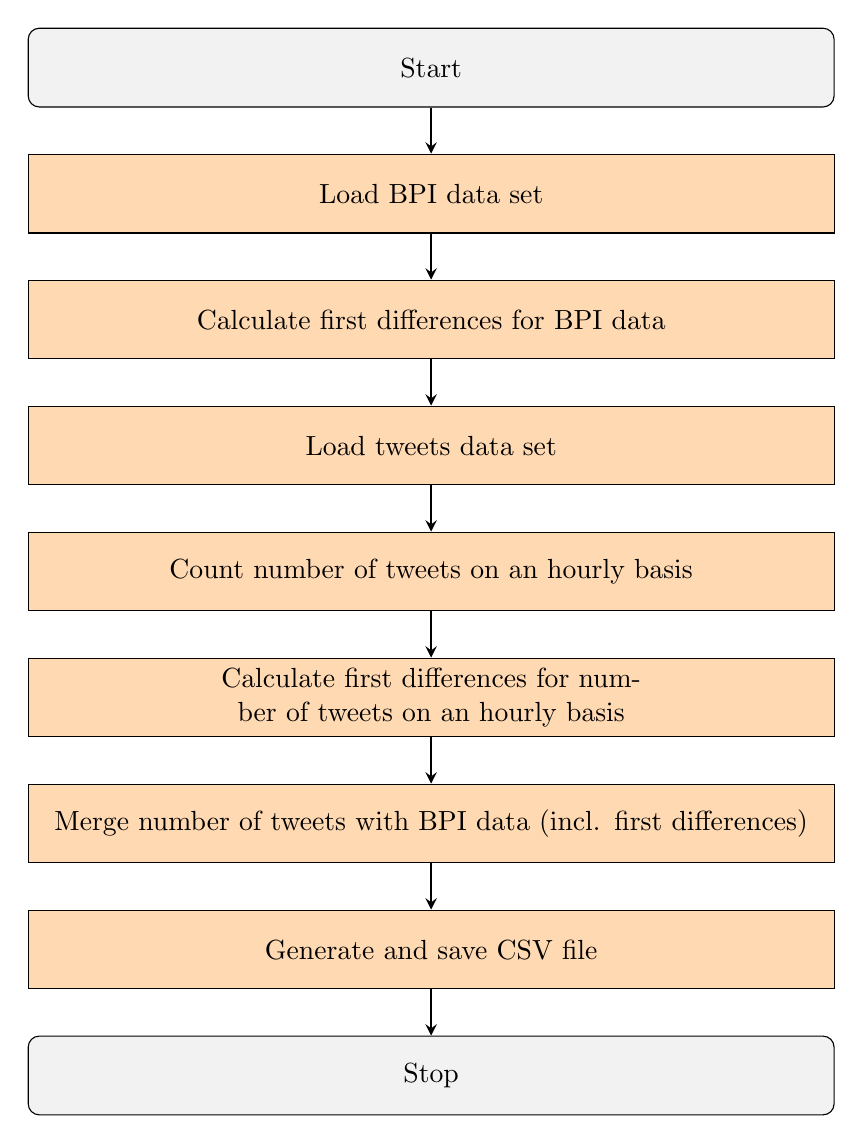
\begin{tikzpicture}[node distance=1.6cm]
        \node (start) [startstop] {Start};
        \node (pro1) [process, below of=start] {Load BPI data set};
        \node (pro2) [process, below of=pro1] {Calculate first differences for BPI data};
        \node (pro3) [process, below of=pro2] {Load tweets data set};
        \node (pro4) [process, below of=pro3] {Count number of tweets on an hourly basis};
        \node (pro5) [process, below of=pro4] {Calculate first differences for number of tweets on an hourly basis};
        \node (pro6) [process, below of=pro5] {Merge number of tweets with BPI data (incl. first differences)};
        \node (pro7) [process, below of=pro6] {Generate and save CSV file};
        \node (stop) [startstop, below of=pro7] {Stop};
        
        \draw [arrow] (start) -- (pro1);
        \draw [arrow] (pro1) -- (pro2);
        \draw [arrow] (pro2) -- (pro3);
        \draw [arrow] (pro3) -- (pro4);
        \draw [arrow] (pro4) -- (pro5);
        \draw [arrow] (pro5) -- (pro6);
        \draw [arrow] (pro6) -- (pro7);
        \draw [arrow] (pro7) -- (stop);
    \end{tikzpicture}
\caption{Data aggregation and data wrangling process} \label{fig:dataaggregation}
\end{figure}

Here is a short description of what happens at the various steps: 
\paragraph{Load BPI data set}\mbox{}\\
The script takes the BPI data set that is located at \verb|data/bpi.csv|. Then, BPI closing prices are added to every data point.

\paragraph{Calculate first differences for BPI data}\mbox{}\\
The first differences of the BPI closing prices and the natural logarithm of the first differences of the BPI closing prices are calculated. The reason for calculating these values is provided in chapter 5 (Data Analysis).

\paragraph{Load tweets data set}\mbox{}\\ 
The script takes the tweets data set that is located at \verb|data/twitterData.csv|.

\paragraph{Count number of tweets on an hourly basis}\mbox{}\\ First, groups the tweets by hour. Second, counts the number of tweets for every hour.

\paragraph{Calculate first differences for number of tweets on an hourly basis}\mbox{}\\ 
The first differences of the number of tweets and the natural logarithm of the first differences of the number of tweets are calculated. Again, the reason for calculating these values is given in chapter 5 (Data Analysis).

\paragraph{Merge number of tweets with BPI data (incl. first differences)}\mbox{}\\
Up to this point, there are the two separate data frames df\_tweets\_per\_hour and df\_bpi. Here is an excerpt of an the two data frames look at this point:

\begin{figure}[H]
    \centering
    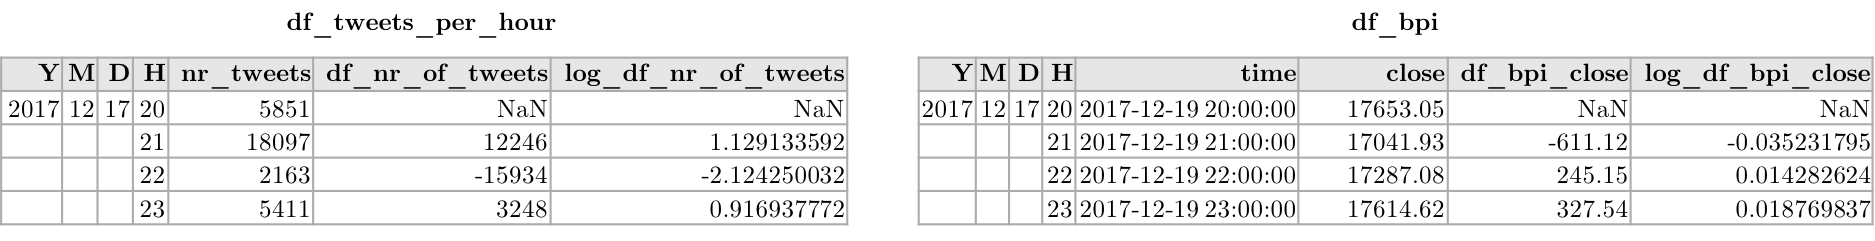
\includegraphics[scale=0.52]{dfseperate.png}
\end{figure}
By using the \verb|pandas.DataFrame.join| function the columns of the \verb|df_tweets_per_hour| are joined with  \verb|df_bpi| on the  \verb|MultiIndex(Y, M, D, H)|. The code snipped for the join \:
\begin{lstlisting}[language=bash]
...
df_merged = df_tweets_per_hour.join(df_bpi, how='left')
...
\end{lstlisting}
An example of the joined data frame looks the following:
\begin{figure}[H]
    \centering
    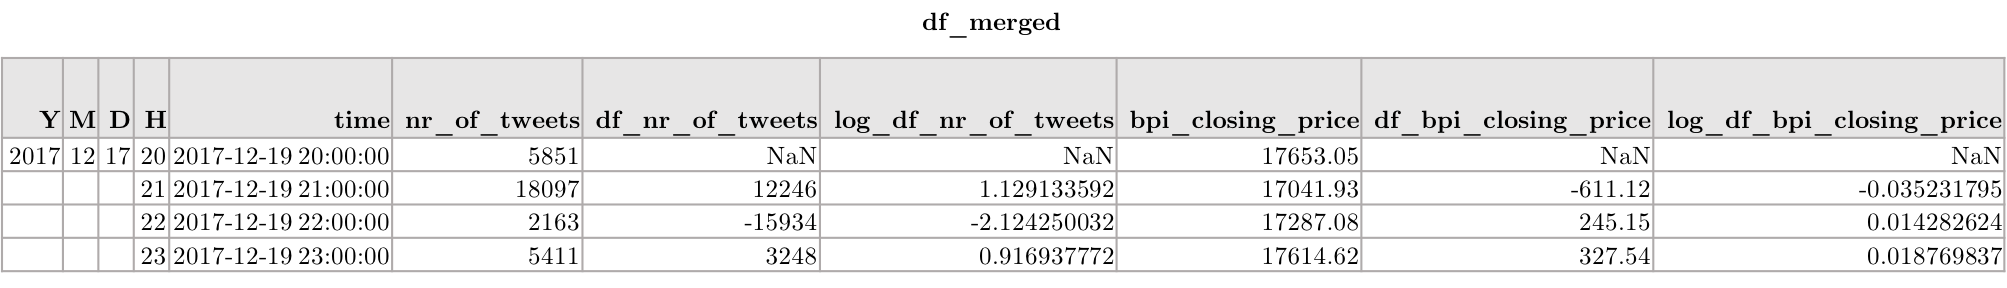
\includegraphics[scale=0.52]{dfmerged.png}
\end{figure}

\subsection{Execution}
By executing the Python script \verb|aggregateTwitterBpi.py| an the aggregated data set that contains number of tweets and Bitcoin Price Index, both on an hourly basis, gets generated. 
\begin{lstlisting}[language=bash]
    $ python aggregateTwitterBpi.py
\end{lstlisting}

\subsection{Output}
After successfully running the Python script \verb|aggregateTwitterBpi.py|, the file \\ \verb|nr_of_tweets_bpi_closing_price.csv| is generated in the folder \verb|/data|. It is important to note that every execution of the script overwrites any existing \\ \verb|nr_of_tweets_bpi_closing_price.csv| file.

The file \verb|aggregateTwitterBpi.csv| contains historical tweets and Bitcoin Price Index data. Each data point consists of the following parameters:
\begin{itemize}
    \item time: Timestamp on an hourly basis in UTC time
    \item {nr\_of\_tweets}: Sum of tweets
    \item {df\_nr\_of\_tweets}: First difference of the sum of tweets
    \item {log\_df\_nr\_of\_tweets}: Natural logarithm of the first difference of the sum of tweets
    \item {bpi\_closing\_price}: BPI closing price
    \item {df\_bpi\_closing\_price}: First difference of the BPI closing price
    \item {log\_df\_bpi\_closing\_price}: Natural logarithm of the first difference of the BPI closing price
\end{itemize}

\clearpage

\section{Data Analysis}
The data analysis was performed with the statistical software STATA (version 14.2). The corresponding .dta file and .do file are stored in the folder  \verb|/documentation/stata_analysis/| in the Github repository. Following, we describe all the commands used to produce our econometric model.

Step 1:\\
After starting STATA the first step was to import the data file (.csv file). We did so by following command (be careful, your location of the .csv file will probably differ):\\
\begin{lstlisting}[language=bash]
    import delimited C:\Users\Dimi\Desktop\nr_of_tweets_bpi_closing_price.csv
\end{lstlisting}

Step 2:\\
STATA is not recognizing our variable "time" as a date variable. Therefore, we had to create a new variable "time2" and give it the same values as "time" in the same format as "time". At the end, we define "time2" to be a time series with an hourly progress.\\
	\begin{lstlisting}[language=bash]
	gen double time2 = clock(time, "YMD hms")\\
	format time2 %tcNN-DD-CCYY_HH:MM:SS\\
	order time2, after(time)\\
	tsset time2, format(%tcNN-DD-CCYY_HH:MM:SS) delta(1 hours)
	\end{lstlisting}

Step 3:\\
Next we plotted all variables by the following commands and exported the produced graphs (and saved in local repository):\\
	\begin{lstlisting}[language=bash]
	twoway (tsline nr_of_tweets)
	twoway (tsline df_nr_of_tweets)
	twoway (tsline log_df_nr_of_tweets)
	twoway (tsline bpi_closing_price)
	twoway (tsline df_bpi_closing_price)
	twoway (tsline log_df_bpi_closing_price)
	\end{lstlisting}

Step 4:\\
To check for stationarity, we run the Augmented Dickey-Fuller (ADF) test for all variables with a time delay of 0 periods (lag 0).\\
	\begin{lstlisting}[language=bash]
	dfuller nr_of_tweets, lags(0)
	dfuller df_nr_of_tweets, lags(0)
	dfuller log_df_nr_of_tweets, lags(0)
	dfuller bpi_closing_price, lags(0)
	dfuller df_bpi_closing_price, lags(0)
	dfuller log_df_bpi_closing_price, lags(0)
	\end{lstlisting}

Step 5:\\
Calling the lag-order selection criteria statistics for our VAR model. The maximum amount of lags is 7 and the variables that we chose for the later VAR model are df\_nr\_of\_tweets and df\_bpi\_closing\_price.\\
	\begin{lstlisting}[language=bash]
	varsoc df_nr_of_tweets df_bpi_closing_price, maxlag(7)
	\end{lstlisting}

Step 6:\\
Running the VAR regression for our two variables. With recommended lag of 1 (from Step 5).\\
	\begin{lstlisting}[language=bash]
	var df_nr_of_tweets df_bpi_closing_price, lags(1/1)
	\end{lstlisting}

Step 7:\\
Calling the granger causality test with lag length 1.\\
	\begin{lstlisting}[language=bash]
	Vargranger
	\end{lstlisting}

Step 8:\\
The VAR regression results were exported to a latex format by installing and using the outreg2 package. The generated piece of latex code was then inserted into in the latex file of the paper. All other results were exported with an image software and used as .png files in latex\\
	\begin{lstlisting}[language=bash]
	ssc install outreg2
	outreg2 using var_gegression_results.tex, replace
	\end{lstlisting}

\end{spacing}
\clearpage

%************************** Bibliography **************************
\section{References}
\printbibliography[heading=none]
\clearpage

%************************** Declaration of Authorship **************************
\section{Declaration of Authorship}
We hereby declare,

\begin{itemize}
	\item that we have written this thesis without any help from others and without the use of documents and aids other than those stated above;
	\item that we have mentioned all the sources used and that we have cited them correctly according to established academic citation rules;
    \item that we have acquired any immaterial rights to materials we may have used such as images or graphs, or that we have produced such materials ourself;
    \item that the topic or parts of it are not already the object of any work or examination of another course unless this has been explicitly agreed on with the faculty member in advance and is referred to in the thesis;
    \item that we are aware that our work can be electronically checked for plagiarism and that we hereby grant the University of St.Gallen copyright in accordance with the Examination Regulations in so far as this is required for administrative action;
    \item that we are aware that the University will prosecute any infringement of this declaration of authorship and, in particular, the employment of a ghostwriter, and that any such infringement may result in disciplinary and criminal consequences which may result in our expulsion from the University or us being stripped of our degree.
\end{itemize}

\begin{flushleft}
Alen Stepic - 11-475-258\\\bigskip\bigskip  
Dimitrios Koumnakes - 10-613-370\\\bigskip\bigskip
Severin Kranz - 13-606-355\\\bigskip\bigskip
Joël Sonderegger - 11-495-488\\\bigskip\bigskip
Chi Xu - 16-300-915

By submitting this academic term paper, we confirm through my conclusive action that we are submitting the Declaration of Authorship, that we have read and understood it, and that it is true.

\end{flushleft}
\clearpage

%************************** DOCUMENT-END **************************
\end{document}

